%%%%%%%%%%%%%%%%%%%%%%%%%%%%%%%%%%%%%%%%%
% Jacobs Landscape Poster
% LaTeX Template
% Version 1.1 (14/06/14)
%
% Created by:
% Computational Physics and Biophysics Group, Jacobs University
% https://teamwork.jacobs-university.de:8443/confluence/display/CoPandBiG/LaTeX+Poster
% 
% Further modified by:
% Nathaniel Johnston (nathaniel@njohnston.ca)
%
% This template has been downloaded from:
% http://www.LaTeXTemplates.com
%
% License:
% CC BY-NC-SA 3.0 (http://creativecommons.org/licenses/by-nc-sa/3.0/)
%
%%%%%%%%%%%%%%%%%%%%%%%%%%%%%%%%%%%%%%%%%

%----------------------------------------------------------------------------------------
%	PACKAGES AND OTHER DOCUMENT CONFIGURATIONS
%----------------------------------------------------------------------------------------

\documentclass[final]{beamer}

\usepackage[scale=1.24]{beamerposter} % Use the beamerposter package for laying out the poster

\usetheme{confposter} % Use the confposter theme supplied with this template

\setbeamercolor{block title}{fg=ngreen,bg=white} % Colors of the block titles
\setbeamercolor{block body}{fg=black,bg=white} % Colors of the body of blocks
\setbeamercolor{block alerted title}{fg=white,bg=dblue!70} % Colors of the highlighted block titles
\setbeamercolor{block alerted body}{fg=black,bg=dblue!10} % Colors of the body of highlighted blocks
% Many more colors are available for use in beamerthemeconfposter.sty

%-----------------------------------------------------------
% Define the column widths and overall poster size
% To set effective sepwid, onecolwid and twocolwid values, first choose how many columns you want and how much separation you want between columns
% In this template, the separation width chosen is 0.024 of the paper width and a 4-column layout
% onecolwid should therefore be (1-(# of columns+1)*sepwid)/# of columns e.g. (1-(4+1)*0.024)/4 = 0.22
% Set twocolwid to be (2*onecolwid)+sepwid = 0.464
% Set threecolwid to be (3*onecolwid)+2*sepwid = 0.708

\newlength{\sepwid}
\newlength{\onecolwid}
\newlength{\twocolwid}
\newlength{\threecolwid}
\setlength{\paperwidth}{48in} % A0 width: 46.8in
\setlength{\paperheight}{36in} % A0 height: 33.1in
\setlength{\sepwid}{0.024\paperwidth} % Separation width (white space) between columns
\setlength{\onecolwid}{0.22\paperwidth} % Width of one column
\setlength{\twocolwid}{0.464\paperwidth} % Width of two columns
\setlength{\threecolwid}{0.708\paperwidth} % Width of three columns
\setlength{\topmargin}{-0.5in} % Reduce the top margin size
%-----------------------------------------------------------

\usepackage{graphicx}  % Required for including images

\usepackage{booktabs} % Top and bottom rules for tables

%----------------------------------------------------------------------------------------
%	TITLE SECTION 
%----------------------------------------------------------------------------------------

\title{ETERNITY: NUMBERS - Silver Ratio $(\delta_s)$} % Poster title

\author{Md Hasibul Huq} % Author(s)

\institute{Department of Computer Science and Software Engineering (CSSE) , Concordia University} % Institution(s)

%----------------------------------------------------------------------------------------

\begin{document}

\addtobeamertemplate{block end}{}{\vspace*{2ex}} % White space under blocks
\addtobeamertemplate{block alerted end}{}{\vspace*{2ex}} % White space under highlighted (alert) blocks

\setlength{\belowcaptionskip}{2ex} % White space under figures
\setlength\belowdisplayshortskip{2ex} % White space under equations

\begin{frame}[t] % The whole poster is enclosed in one beamer frame

\begin{columns}[t] % The whole poster consists of three major columns, the second of which is split into two columns twice - the [t] option aligns each column's content to the top

\begin{column}{\sepwid}\end{column} % Empty spacer column

\begin{column}{\onecolwid} % The first column

%----------------------------------------------------------------------------------------
%	OBJECTIVES
%----------------------------------------------------------------------------------------

\begin{alertblock}{Objectives}

The objective of this project is develop a document of software requirement specification to learn how the industry runs it's operation. Tried to develop a SRS  based on specific criteria. Those are:- 
\begin{itemize}
\item Learn about an irrational number.
\item Interviewing someone related to the specific assigned number
\item Based on the interview analyze the interview. 
\item Develop a Class diagram, a use case diagram, and an activity diagram based on the analysis.
\item Find out user stories from the above mention sources and out of the mention list .
\item Based on the user stories tractability matrix creation
\item Developing a calculator based on the user stories. 
\end{itemize}
The main objective of this project is to integrate the necessary  operation that is not available in calculator but need to support this numbers in calculator.
\end{alertblock}

%----------------------------------------------------------------------------------------
%	INTRODUCTION
%----------------------------------------------------------------------------------------

\begin{block}{Introduction}

This poster provides an understanding of only an irrational  number called Silver Ratio $(\delta_s)$. An irrational  number is  not  a rational  number, it is not possible to express an irrational number as a quotient of two integers \cite{project_des}.

\end{block}

%------------------------------------------------

\begin{figure}
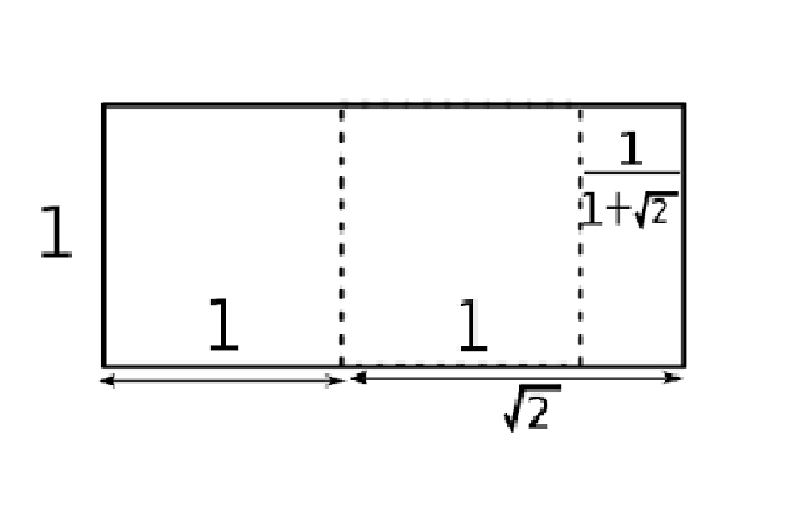
\includegraphics[width=0.8\linewidth]{silver_ratio.png}
\caption{Silver Rectangle}
\end{figure}

%----------------------------------------------------------------------------------------

\end{column} % End of the first column

\begin{column}{\sepwid}\end{column} % Empty spacer column

\begin{column}{\twocolwid} % Begin a column which is two columns wide (column 2)

\begin{columns}[t,totalwidth=\twocolwid] % Split up the two columns wide column

\begin{column}{\onecolwid}\vspace{-.6in} % The first column within column 2 (column 2.1)

%----------------------------------------------------------------------------------------
%	History
%----------------------------------------------------------------------------------------

\begin{block}{History}
Silver Ratio is studied from the time of Greek knowledge, which discusses the fundamental characteristics of the number system. Though it is not used by normal people intentionally. Silver ratio is the limiting of consecutive  of infinite sequence of integers, The silver ratio is presented in a Greek symbol ($\delta_s$).

\end{block}


%----------------------------------------------------------------------------------------

%----------------------------------------------------------------------------------------
%	MATHEMATICAL SECTION
%----------------------------------------------------------------------------------------
\begin{block}{Mathematical Definition}
The value of silver ration is 2.4142135623 \cite{jdc_silver}. A ratio of the sequential sum of smaller number and twice of the larger number, which will produce an infinite sequence and the ration between smaller and larger number will be always same \cite{numberphile_silver}. This can be presented in mathematical equation:- 

\[ \dfrac{2a + b}{a}  = \dfrac{b}{a} = \delta_s \]

It will be easier to understand if it can be compared with Fibonacci number.
In Fibonacci, the smaller and larger number are added to get the next one. 
Example:-

$$1,1,2,3,5,8,13,..$$

For silver ratio, the smaller and twice of the larger number are added to get the next one. Example:-

\[1,2,5,12,29,70,..\] 

Then the latest number is divided  by the previous larger number. 
\end{block}

%----------------------------------------------------------------------------------------
%	Persona
%----------------------------------------------------------------------------------------

\begin{block}{Lesson Learned}

\begin{itemize}
\item Learn about an geometrical uses of irrational numbers.
\item How to conduct a interview.
\item How to Analyze an interview. 
\item Developing UML and Class diagram in 
\item learned different equations to find Silver ratio
\item Learned about the square triangular numbers, Pell numbers, octagons 
\end{itemize}

\end{block}


%----------------------------------------------------------------------------------------

\end{column} % End of column 2.1

\begin{column}{\onecolwid}\vspace{-.6in} % The second column within column 2 (column 2.2)

%----------------------------------------------------------------------------------------
%	METHODS
%----------------------------------------------------------------------------------------

\begin{block}{Challenges}
 \begin{itemize}
\item Very few people know about the silver ratio.
\item Arranging a group meeting with all at a time.
\item My interviewee never worked with the silver ratio.
\item Finding it's uses in real world is quite difficult
\item Resources related to it is vague 
\item Implementation without build in function makes life herder.
\item Find user intention from an interview is not easy.
\item Find out Software requirements from persons interviewee is difficult.
\end{itemize}
\end{block}

\begin{block}{How the Challenges are overcome?}
 \begin{itemize}
\item By questioning related known problems.
\item By learning from her theoretical knowledge .
\item By searching on internet.
\item By assuming some information from the internet. 
\item By building an algorithm which gives approximate result.
\item By researching the interview answers.
\item By using the related system.
\end{itemize}
\end{block}

\begin{block}{Critical Decision}
Silver ration has good number of implication in the field of mathematics. Most of the time normal people use those without knowing about it. The ratio is used mainly in the architecture design. 
\begin{figure}
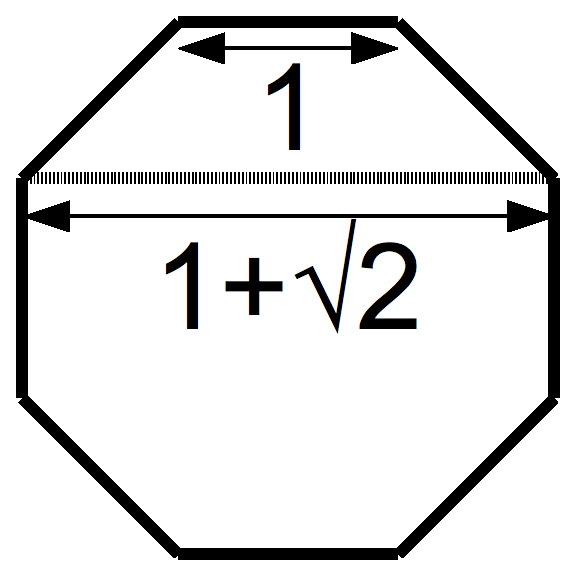
\includegraphics[width=0.3\linewidth]{silver_ratio_octagon.png}
\caption{Silver Rectangle}
\end{figure}
From the uses of silver ratio I chose to implement to find the ratio of a given number. Which will help to draw shapes based on the proportioned number. As an example silver rectangle and octagon. 
\end{block}
%----------------------------------------------------------------------------------------

\end{column} % End of column 2.2

\end{columns} % End of the split of column 2 - any content after this will now take up 2 columns width

%----------------------------------------------------------------------------------------
%	IMPORTANT RESULT
%----------------------------------------------------------------------------------------



%----------------------------------------------------------------------------------------

\end{column} % End of the second column

\begin{column}{\sepwid}\end{column} % Empty spacer column

\begin{column}{\onecolwid} % The third column


%----------------------------------------------------------------------------------------
%	CONCLUSION
%----------------------------------------------------------------------------------------

\begin{block}{Conclusion}

In this document, how the software requirements specification document are created , what are the challenges faced during the project and how they are solved is mentioned. Also what are the learning's from the project is mentioned. 
More research and good knowledge on the engineering methods can make this projects more accurate and enriched.   

\end{block}

%----------------------------------------------------------------------------------------
%	REFERENCES
%----------------------------------------------------------------------------------------

\begin{block}{References}
\nocite{*} % Insert publications even if they are not cited in the poster
\small{\bibliographystyle{unsrt}
\bibliography{sample}\vspace{0.0in}}
\end{block}
%----------------------------------------------------------------------------------------
%	ACKNOWLEDGEMENTS
%----------------------------------------------------------------------------------------

\setbeamercolor{block title}{fg=red,bg=white} % Change the block title color
\begin{block}{Online Versions}
\begin{itemize}
\item \textbf{Report:} \url{https://github.com/Hasib-rafi1/SRS-Silver-Ratio}
\item \textbf{Project:} \url{https://github.com/Hasib-rafi1/srs-project-calculator}
\end{itemize}
\end{block}
\begin{block}{Acknowledgements}
\small{\rmfamily{I like to show my gratitude to the Pankaj Kamtahn to provide the opportunity to learn new things from the project. I also want to thank my group mates for their valuable contribution to the persona.}} \\

\end{block}

%----------------------------------------------------------------------------------------
%	CONTACT INFORMATION
%----------------------------------------------------------------------------------------

\setbeamercolor{block alerted title}{fg=black,bg=norange} % Change the alert block title colors
\setbeamercolor{block alerted body}{fg=black,bg=white} % Change the alert block body colors

\begin{alertblock}{Contact Information}

\begin{itemize}
\item Web: \href{http://www.hasibulhuq.com}{http://www.hasibulhuq.com}
\item Email: \href{mailto:rafi3170@gmail.com}{rafi3170@gmail.com}
\item Phone: +1 (438) 866 7234
\end{itemize}

\end{alertblock}


%----------------------------------------------------------------------------------------

\end{column} % End of the third column

\end{columns} % End of all the columns in the poster

\end{frame} % End of the enclosing frame

\end{document}
